\chapter{Resultate und Testen} \label{chap:resultate}

\section{Testen} \label{sec:testen}

Die Webseite lässt sich testen in einer lokalen Entwicklungsumgebung oder auf
der öffentlichen Seite. Getestet wurden die Funktionen manuell von Hand oder
durch automatisierte Tests.

Grundsätzlich funktionieren alle Funktionen. Schlussendlich gibt es nur ein
Problem: Es kommt vor, dass der Webscraper Edge-Cases antrifft. Das kann
passieren, wenn die offizielle Mensa Webseite die Informationen auf ihrer
Webseite kurzfristig ändern. Es wurde versucht diese Edge-Cases möglichst alle
abzufangen, allerdings kann es immer noch sein, dass es manchmal zu Fehlern
kommt. Diese Fehler müssten dann von einem Admin auf der Admin-Seite behoben
werden.

\section{Resultate} \label{sec:resultate}

Als Resultat dieser Arbeit ist eine voll funktionsfähige Webseite entstanden.
Die Webseite erfüllt alle nötigen Anforderungen (siehe
\ref{sec:problemdefinition}). Die Webseite ist auch öffentlich zugänglich
(siehe \ref{spez:Deployment}) und kann unter
\url{http://mensarating.herokuapp.com/} aufgerufen werden. Es lässt sich also
sagen, dass die Webseite komplett einsatzbereit ist und Nutzer von der NKSA sie
beginnen können zu benutzen.

\subsection{Resultate der Grundanforderungen}
 
\newpage

\subsubsection*{Anzeige der Menus}

\begin{figure}[ht]
    \centering
    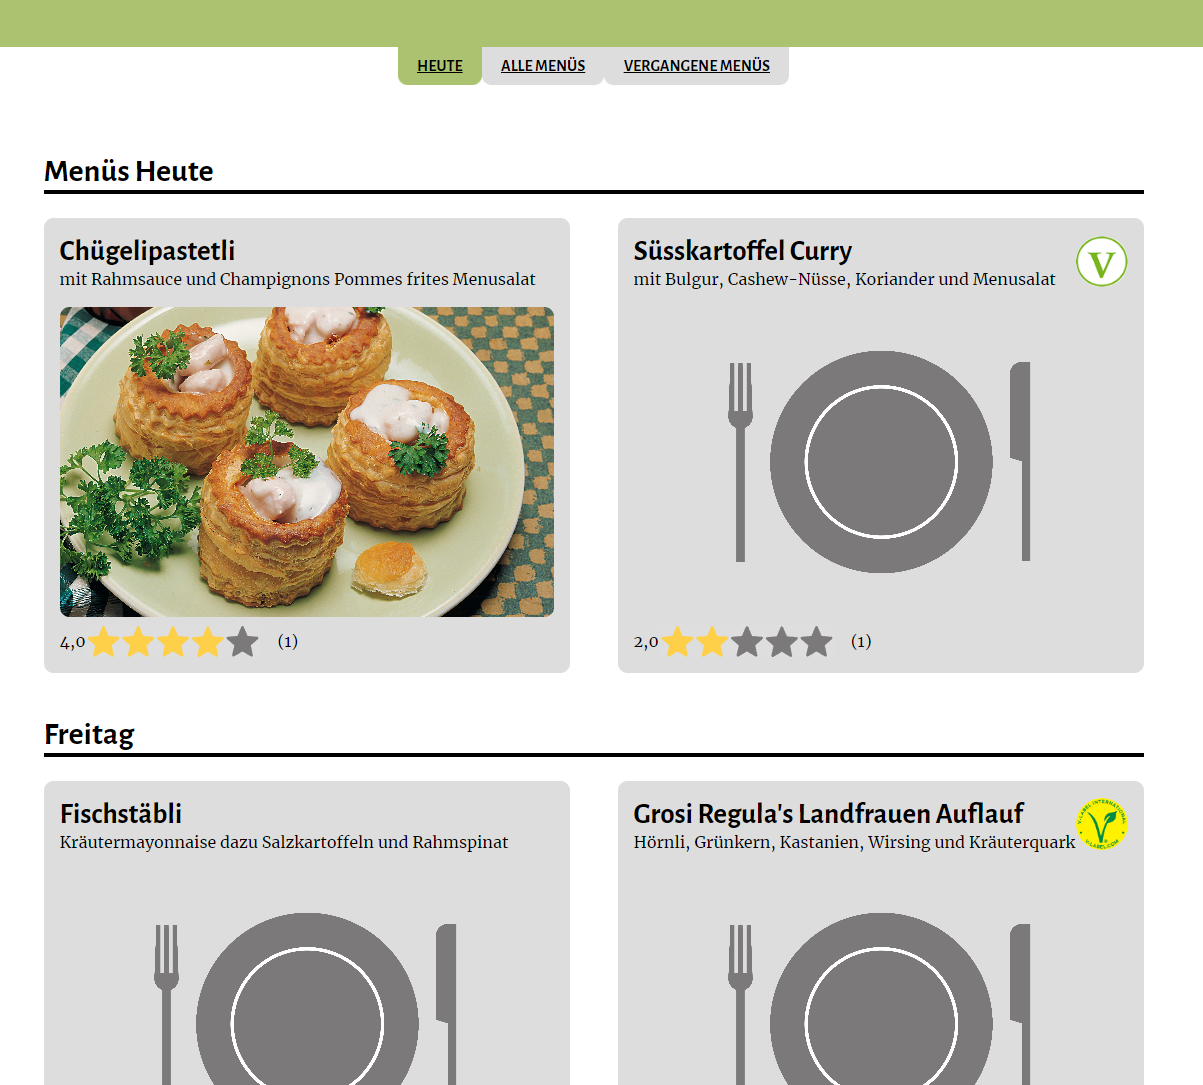
\includegraphics[width=0.8\textwidth]{images/Resultate_Menu.png}
    \caption{Screenshot: Anzeige Menus auf Startseite}
    \label{fig:r-menuindex}
\end{figure}

Auf der Startseite der Webseite (siehe \ref{fig:r-menuindex}) werden die beiden Menus des Tages, die von der
offiziellen Mensa Webseite gescraped wurden, angezeigt. Es wird die
Beschreibung, ein Label (Vegan/Vegetarisch), das durchschnittliche Rating und
das Bild mit den meisten Likes angezeigt. Als Zusatz sind die zukünftigen Menus
ebenfalls angezeigt

\begin{figure}[htp]
    \begin{subfigure}[b]{0.5\textwidth}
        \centering
        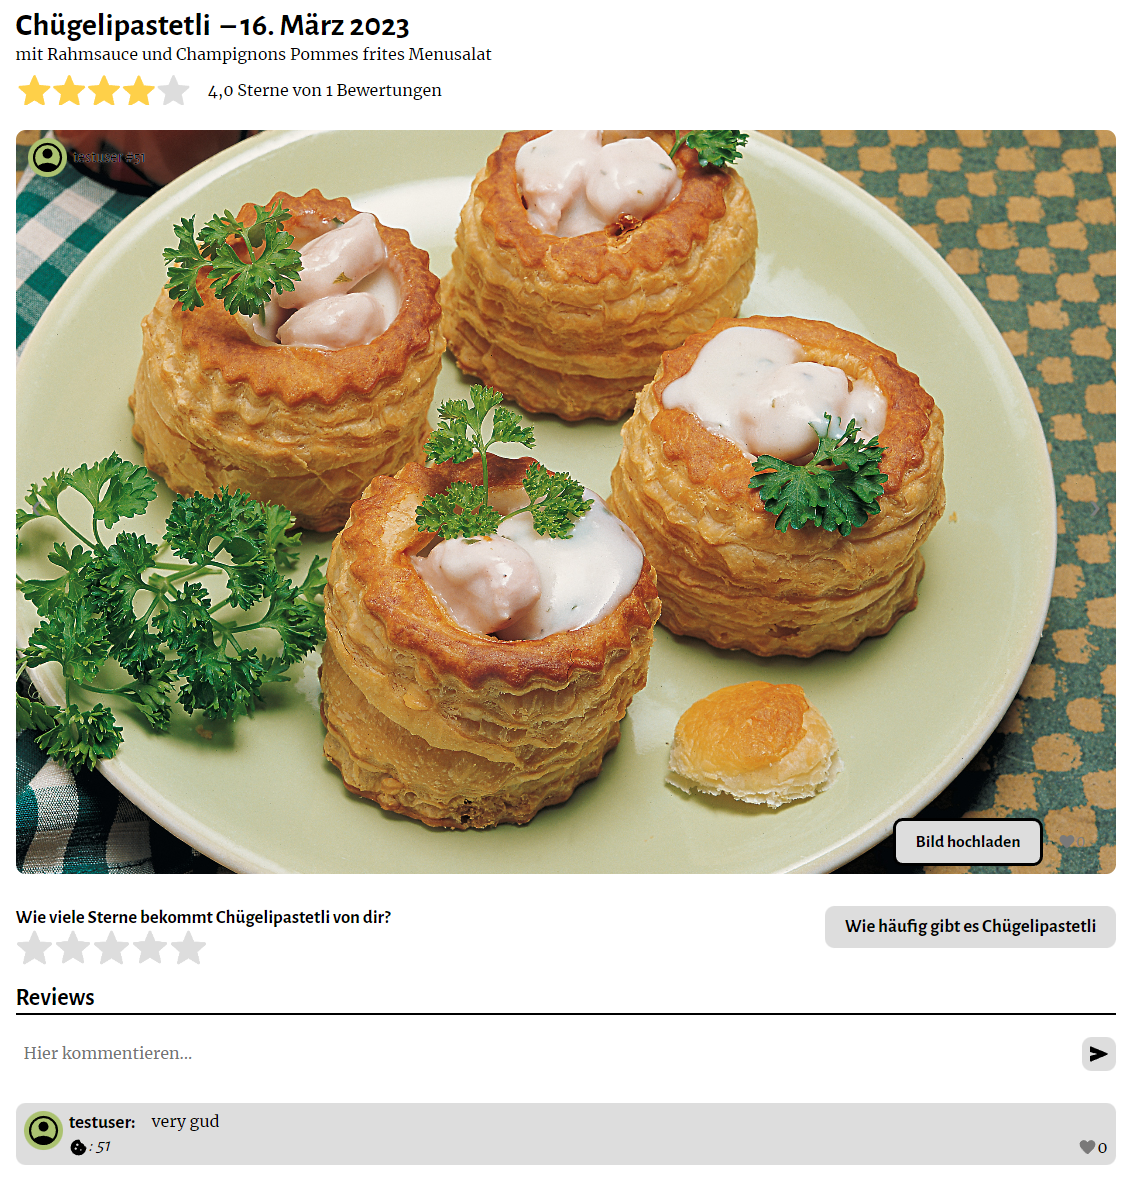
\includegraphics[width=0.7\textwidth]{images/Res_Menu.png}
        \caption{Screenshot: Menu Web Page}
        \label{fig:r-menu}
    \end{subfigure}
    \begin{subfigure}[b]{0.5\textwidth}
        \centering
        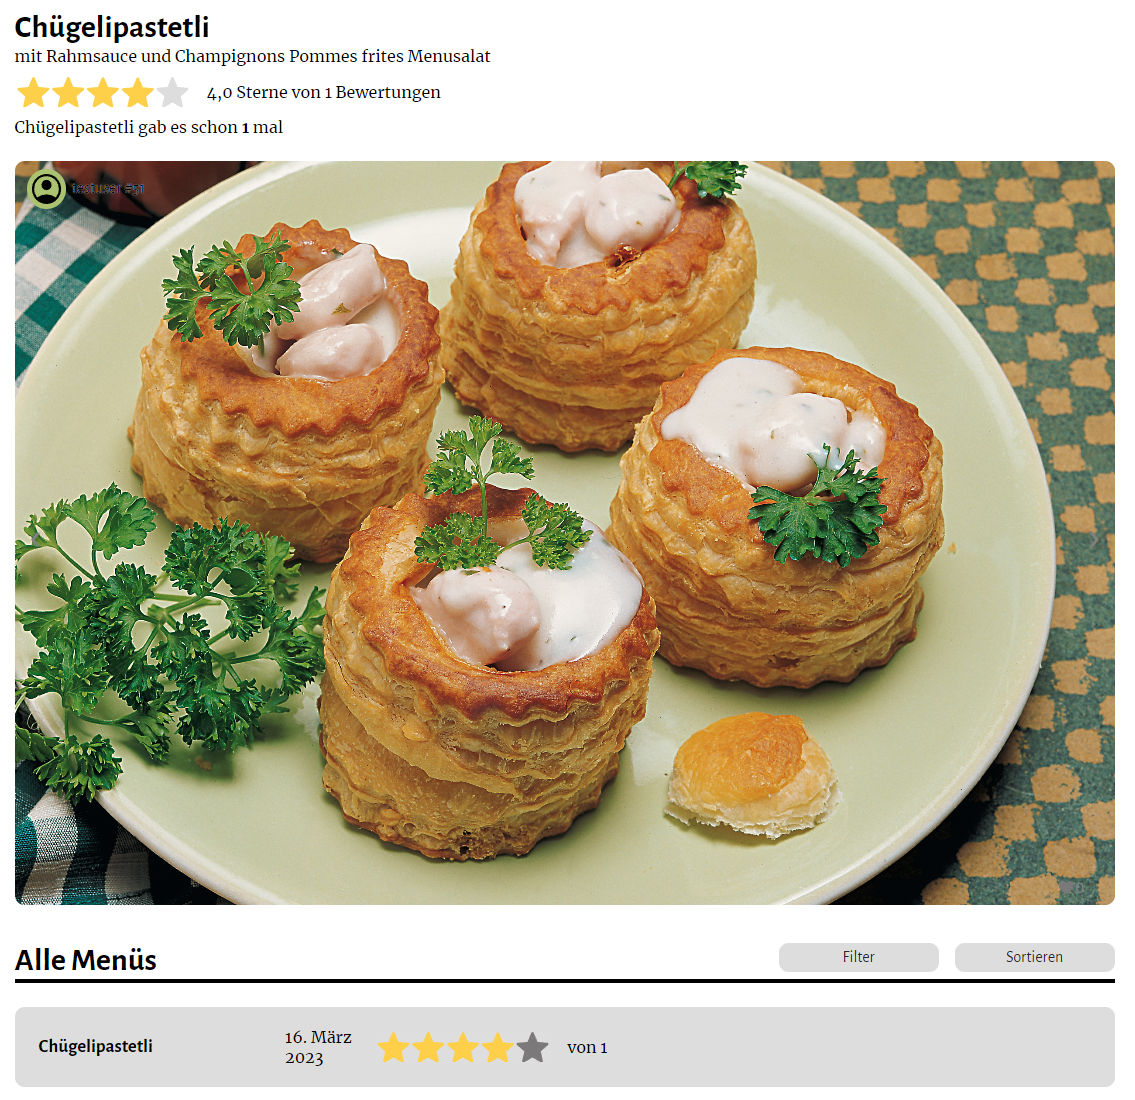
\includegraphics[width=0.7\textwidth]{images/Res_Menutype.png}
        \caption{Screenshot: Menutype Web Page}
        \label{fig:r-menutype}
    \end{subfigure}
    \hfill
\end{figure}

Zusätzlich gibt es eine Menu Page (siehe \ref{fig:r-menu}) und eine MenuType
Page (siehe \ref{fig:r-menutype}), wo die Menus genauer angezeigt werden  


\subsubsection*{Bilder Gallerie}

\begin{figure}[htp]
    \begin{subfigure}[b]{0.5\textwidth}
        \centering
        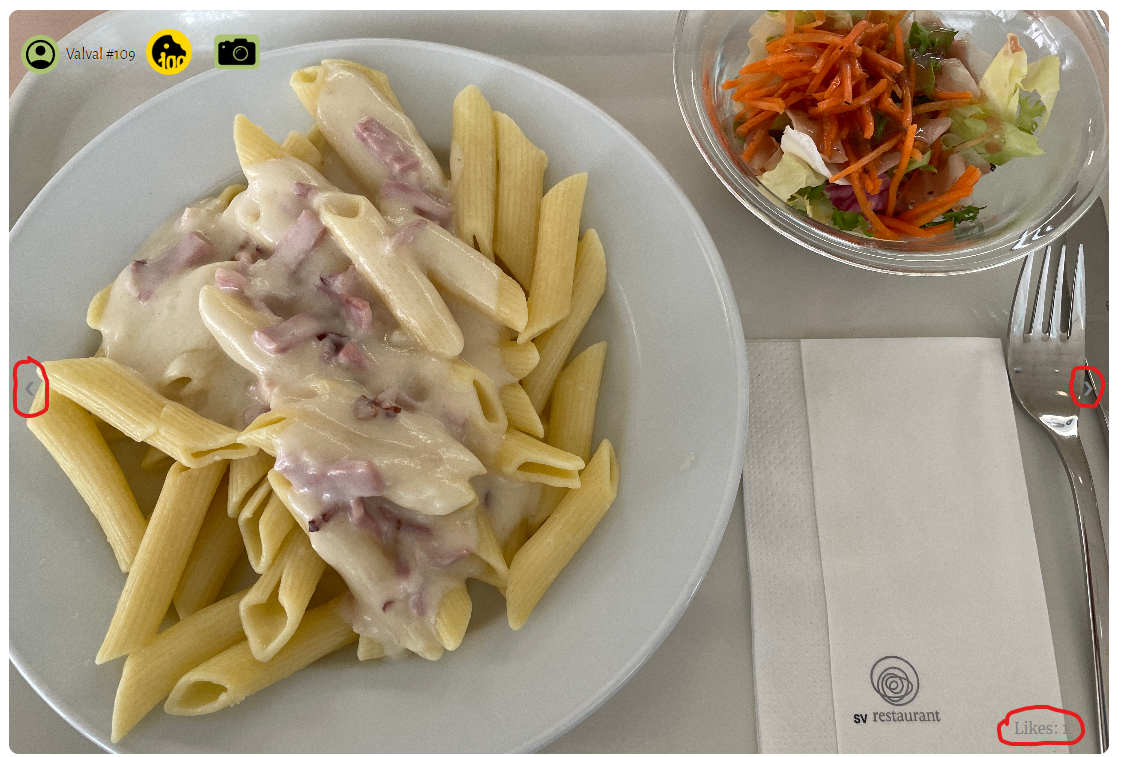
\includegraphics[width=0.7\textwidth]{images/Resultate_Bildergallerie.png}
        \caption{Screenshot: Bildergallerie}
        \label{fig:r-bildergallerie}
    \end{subfigure}
    \begin{subfigure}[b]{0.5\textwidth}
        \centering
        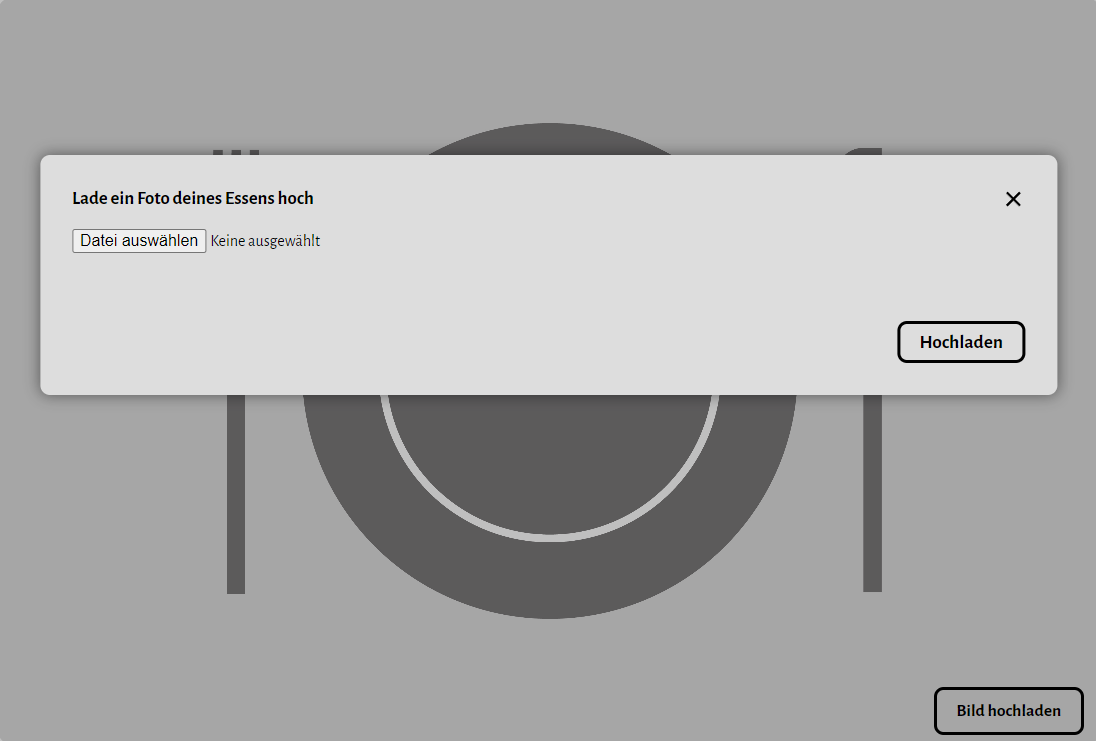
\includegraphics[width=0.7\textwidth]{images/Resultat_Bildergallerie_upload.png}
        \caption{Screenshot: Bilder Upload}
        \label{fig:r-bildpopup}
    \end{subfigure}
    \hfill
\end{figure}

Bei der Bildergallerie (siehe \ref{fig:r-bildergallerie}) können User Bilder
hochladen. Man kann durch Pfeil-Buttons die hochgeladenen Bilder durchschauen.
Für ein Bild ist der User angezeigt, der es hochgeladen hat, und die Anzahl
likes. Der Upload findet über einen Upload Button statt, der ein Pop-Up öffnet
(siehe \ref{fig:r-bildpopup})


\subsubsection*{Reviews}

\begin{figure}[ht]
    \centering
    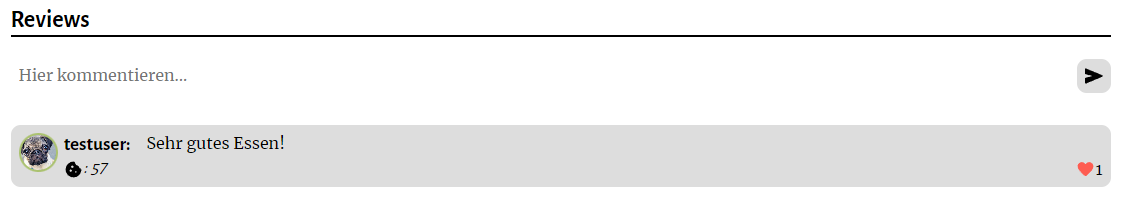
\includegraphics[width=0.8\textwidth]{images/Resultat_Review.png}
    \caption{Screenshot: Veröffentlichung und Anzeige von Reviews}
    \label{fig:r-review}
\end{figure}

Am Tag, an dem es ein Menu gibt, kann diesem Menu ein Review (siehe \ref{fig:r-review}) gegeben werden. Die
Reviews sind in einer Liste angeordet und bei jedem Review ist der User
angegeben, zusammen mit seinen Achievements und Karma Punkten. Reviews können
geliked werden (Beachte das Herz).


\subsubsection*{Rating}

\begin{figure}[ht]
    \centering
    
\includegraphics[width=0.8\textwidth]{images/Resultat_Rating.png}
    \caption{Screenshot: Anzeige vom Rating eines Menus}
    \label{fig:r-rating}
\end{figure}

Ein User kann einem Menu als Rating eienen bis fünf Sterne gebe. Der User drückt
dabei auf die anzahl sterne, die er geben will. Der Durchschnitt des Ratings
wird ebenfalls in der Form von Sternen angezeigt. Dabei kann es auch nicht volle
Sterne geben (siehe \ref{fig:r-rating}) 

\subsubsection*{Filtern/Sortieren}

\begin{figure}[ht]
    \centering
    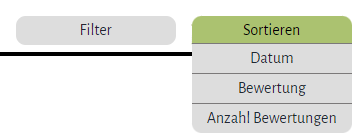
\includegraphics[width=0.8\textwidth]{images/Resultat_Filter.png}
    \caption{Screenshot: Buttons für Filter- und Sortier-Optionen}
    \label{fig:r-filtersort}
\end{figure}

auf der `Alle Menüs' Page und der `MenuType' Page können die Menüs/MenuTypes
nach verschiedenen Optionen in einem Dropdown-Menu (siehe
\ref{fig:r-filtersort}) gefiltert/sortiert werden. Nach der Auswahl wird die
Aktion ohne einen Reload der Seite ausgeführt.

\subsubsection*{Design}
Das Design ist an allen bisherigen Screenshots erkennbar. Als Akzentfarbe wurde
ein Grün gewählt, an vielen Formen sind die Ecken abgerundet und die
verschiedenen Aktionen auf der Webseite sollten für den User so einfach wie
möglich gestaltet sein



\subsection{Resultate der Erweiterungskriterien}

\subsubsection*{Account System}

\begin{figure}[htp]
    \begin{subfigure}[b]{0.32\textwidth}
        \centering
        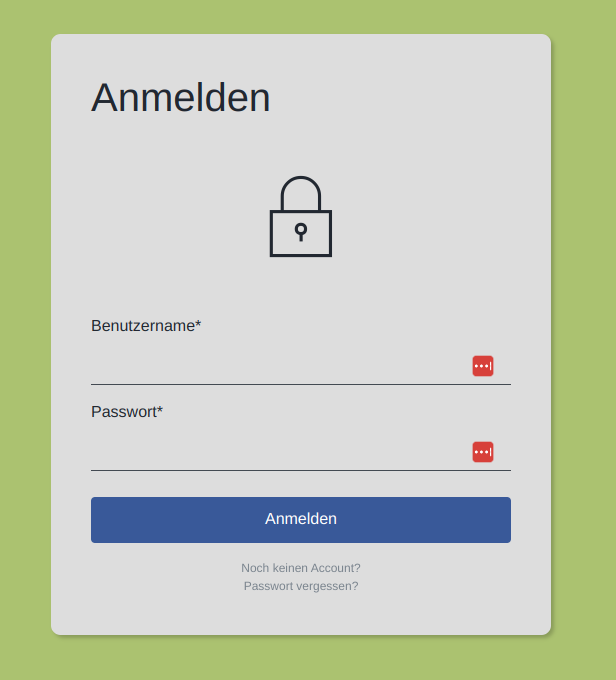
\includegraphics[width=0.7\textwidth]{images/Auth1.png}
        \caption{Screenshot: Login Form}
        \label{fig:r-login}
    \end{subfigure}
    \begin{subfigure}[b]{0.32\textwidth}
        \centering
        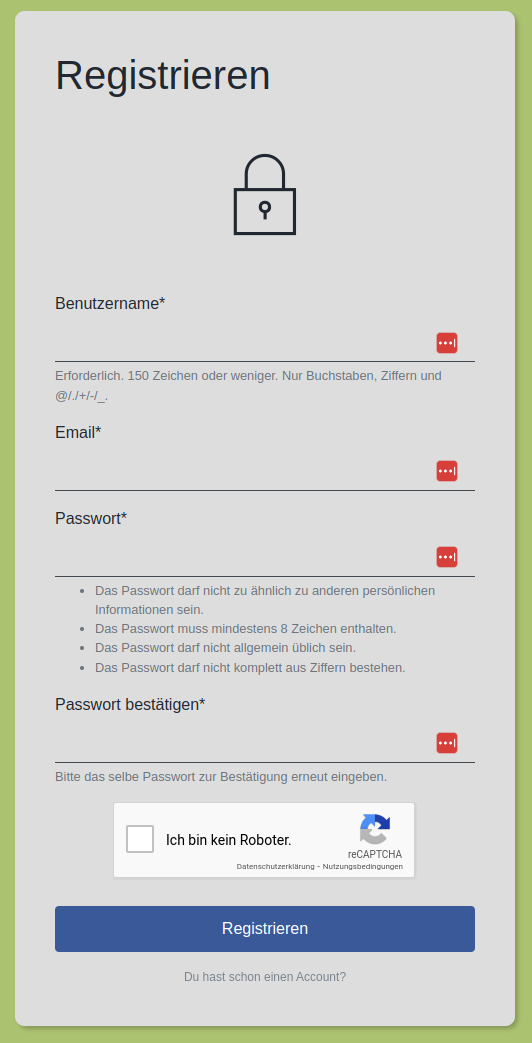
\includegraphics[width=0.7\textwidth]{images/Auth2.png}
        \caption{Screenshot: Registrieren Form}
        \label{fig:r-register}
    \end{subfigure}
    \begin{subfigure}[b]{0.32\textwidth}
        \centering
        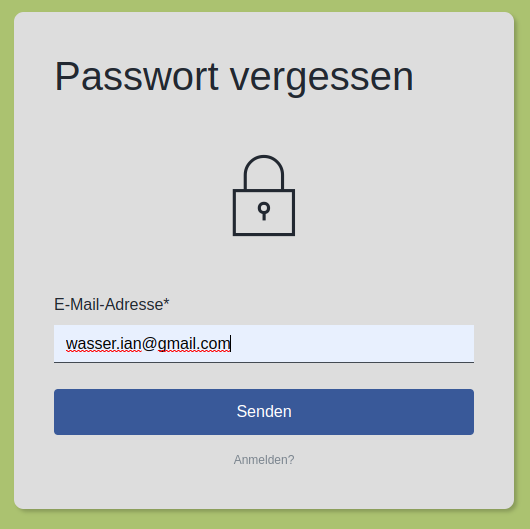
\includegraphics[width=0.7\textwidth]{images/Auth3.png}
        \caption{Screenshot: Passwort Reset Form}
        \label{fig:r-reset}
    \end{subfigure}
    \begin{subfigure}[b]{\textwidth}
        \centering
        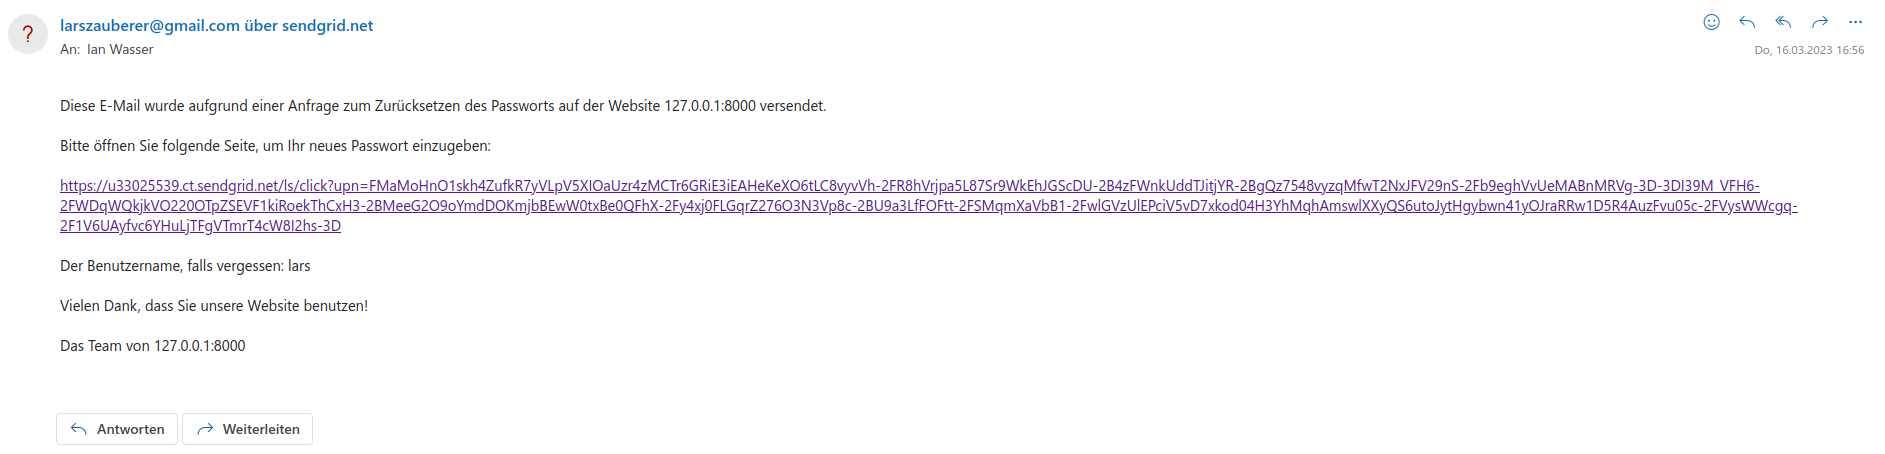
\includegraphics[width=\textwidth]{images/Auth4.png}
        \caption{Screenshot: Passwort Reset Mail}
        \label{fig:r-reset-mail}
    \end{subfigure}
    \begin{subfigure}[b]{\textwidth}
        \centering
        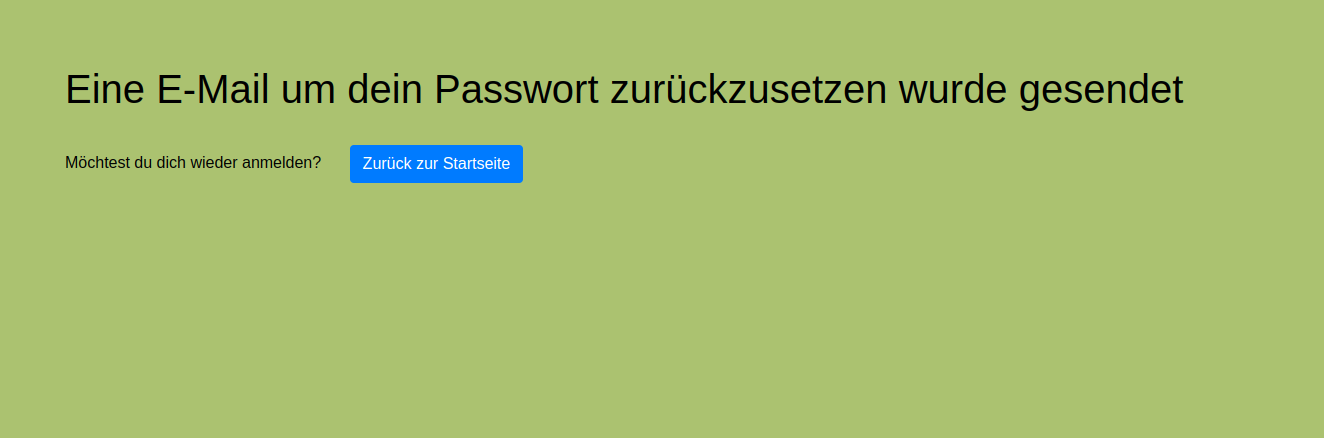
\includegraphics[width=\textwidth]{images/Auth5.png}
        \caption{Screenshot: Passwort Reset Complete}
        \label{fig:r-reset-complete}
    \end{subfigure}
    \caption{Screenshots: Account System}
    \label{fig:r-auth}
\end{figure}

Die Webseite verfügt über ein komplett funktionierendes Account System. Wie den
einzelnen Screenshots zu entnehmen, kann der User sich registrieren, einloggen,
ausloggen und sein Passwort zurücksetzen.

\subsubsection*{Mobile Responsiveness}

\subsubsection*{Punktesystem (Karma)}

\begin{figure}[ht]
    \centering
    
\includegraphics[width=0.5\textwidth]{images/Resultat_Karma.png}
    \caption{Screenshot: Karma eines Users (Auf Profilseite)}
    \label{fig:r-karma}
\end{figure}

User erhalten für Interaktionen auf der Webseite so genannte Cookiepoints. Das
Geben eines Ratings gibt einen Cookiepoint und das Hochladen eines Bildes oder
Reviews gibt 5 Cookiepoints. Wenn ein Post geliked wird (siehe
\ref{spez:Posts}), erhält der User, der geposted hat, einen Cookiepoint. 


\begin{figure}[ht]
    \centering
    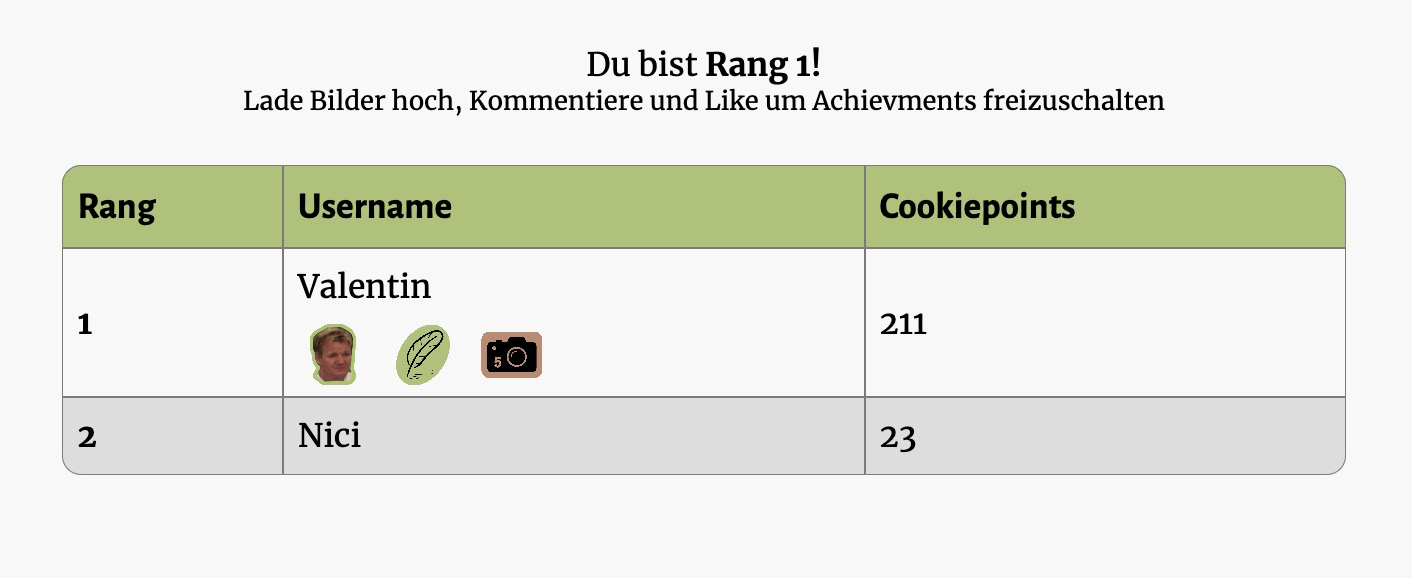
\includegraphics[width=0.8\textwidth]{images/Resultat_Rangliste.png}
    \caption{Screenshot: Karma Rangliste}
    \label{fig:r-rangliste}
\end{figure} 

Alle User mit Account sind in einer Rangliste angegeben. Die Rangliste bezieht
sich auf die Cookiepoints. Der User hat eine Angabe, wo er sich auf der
Rangliste befindet.

\subsubsection*{Achievement System}
\subsubsection*{Deployment}

\begin{figure}[ht]
    \centering
    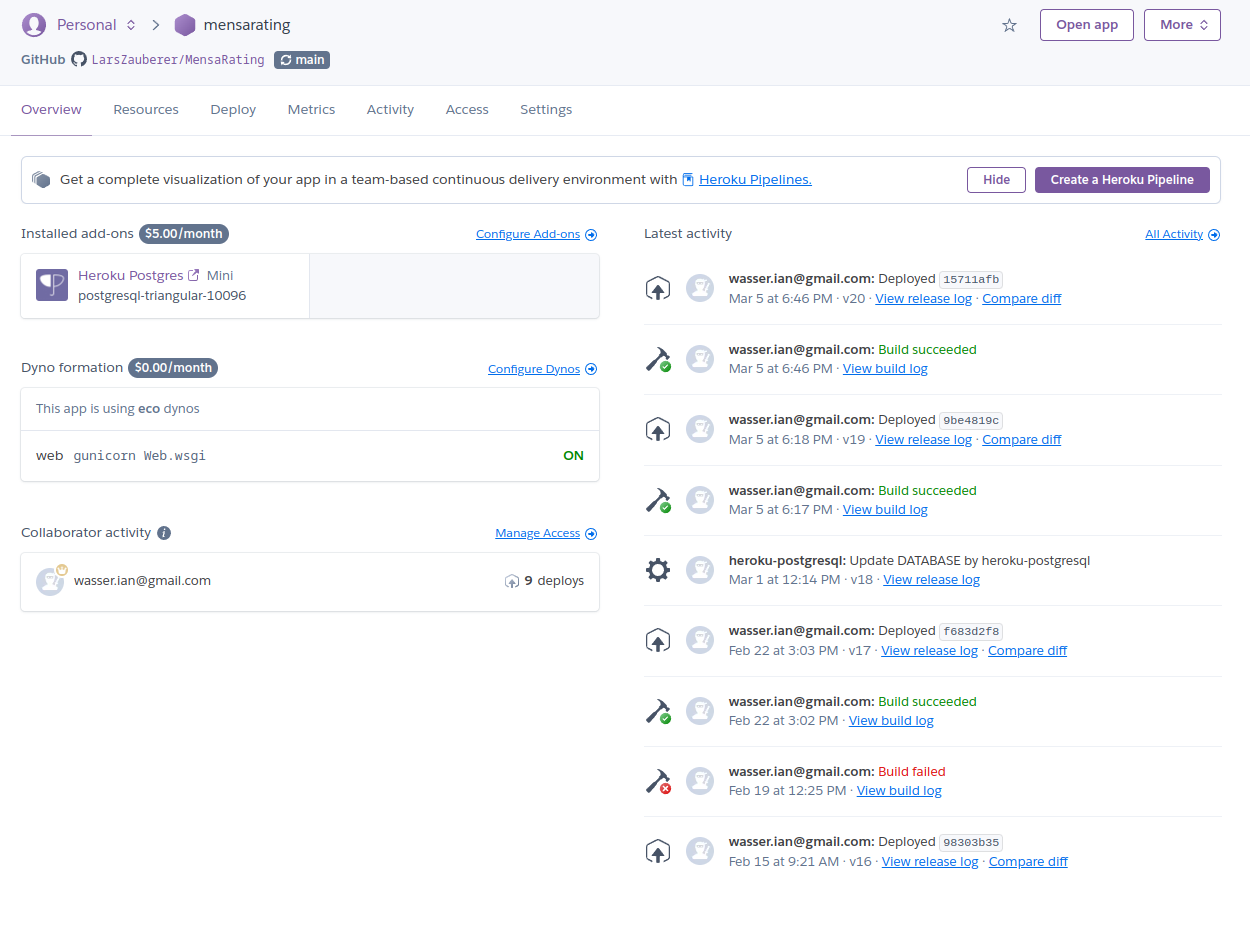
\includegraphics[width=0.8\textwidth]{images/Heroku.png}
    \caption{Screenshot: Heroku Interface für die App}
    \label{fig:r-deployment}
\end{figure}

Die Webseite wurde auf Heroku mit einem Eco-Server und einer Postgres Datenbank
veröffentlicht.




